\documentclass[10pt,a4paper]{article}
\usepackage[margin=1in]{geometry}
\usepackage[T1]{fontenc}
\usepackage{lmodern}
\usepackage{microtype}
\usepackage{amsmath,amssymb,booktabs,array,multirow}
\usepackage{graphicx}
\usepackage[numbers,sort&compress]{natbib}
\usepackage[font=small,labelfont=bf]{caption}
\usepackage{enumitem}
\usepackage{xcolor}
\usepackage[colorlinks=true,linkcolor=blue!50!black,citecolor=blue!50!black,urlcolor=blue!50!black]{hyperref}
\usepackage[section]{placeins}
\usepackage{xurl}
\urlstyle{same}
\renewcommand{\bibfont}{\small}
\setlist{nosep,leftmargin=*}
\setlength{\emergencystretch}{2em}
\widowpenalty=10000
\clubpenalty=10000
\displaywidowpenalty=10000
\newcommand{\mn}{\mbox{MergeNet}}
\newcommand{\pp}{\,pp}
% Requested author working-draft slots; these macros supply no result values.
\newcommand{\pendingvalue}{\rule{0.8cm}{0.3pt}}
\newcommand{\pendingtext}{\par\noindent\textit{Result and interpretation:}\par
  \noindent\rule{0.94\linewidth}{0.3pt}\par\vspace{0.6em}
  \noindent\rule{0.94\linewidth}{0.3pt}\par}
\newcommand{\pendingslot}[3]{\par\medskip\noindent
  \textcolor{blue!55!black}{\textbf{Evidence pending [#1]: #2}}\par
  \noindent\textit{#3}\par\smallskip}
\newcommand{\pendingfigure}[2]{\par\smallskip\noindent
  \fbox{\parbox[c][#2][c]{\dimexpr\linewidth-2\fboxsep-2\fboxrule\relax}{
    \centering\textcolor{gray}{#1}\par\smallskip
    \textcolor{gray}{Reserved space; no measurements or images supplied.}}}\par}

\title{MergeNet: Spatial Routing Gains and Deployment Tradeoffs in Learned Token Compression}
\author{Anonymous authors}
\date{}
\begin{document}
\maketitle
% \begin{abstract}
% Vision transformers retain fine image detail but pay to process every patch
% through every layer. Token merging reduces this cost only when a trainable
% merging policy also produces the shorter tensor used by downstream blocks.
% We introduce \mn{}, a local-to-latent vision transformer that separates these
% roles: continuous spatial mass routing learns where information should flow,
% and an exact-budget gather physically reduces $N$ patches to $K$ carriers
% before global reasoning. Routing is restricted to the original image grid,
% but similarities, transported mass, and carrier locations remain learned. A
% threshold-based soft top-$k$ relaxation trains the routing scores, while a
% straight-through carrier weight connects them to the hard gather. Selected
% mass is retained as a logarithmic key bias; we also give an exact rank-one
% query/key augmentation that implements this bias with an unmodified
% FlashAttention kernel. On ImageNet-1K with DeiT-S/8, the trained checkpoint
% reaches 81.368\% top-1 at $2\times$ carrier compression, versus 82.246\% for
% the dense model; matched-budget evaluation gives 81.360\% for \mn{} and
% 81.932\% for post-training ToMe. Radius-3 routing improves a matched
% 150-epoch control by 1.670 percentage points over global routing and 0.598
% over flattened windows, and three-seed CIFAR-100 controls retain the spatial
% advantage after matching receiver degree. The remaining
% \pendingresult{DTEM score}, \pendingresult{latency}, and
% \pendingresult{memory} cells are explicitly reserved for one common-protocol
% checkpoint evaluation.
% \end{abstract}

\begin{abstract}
Modern visual recognition requires models to capture both fine-grained image
detail and long-range context. Vision transformers meet these needs by
representing images as patch tokens and modeling their interactions, but
retaining every token across layers becomes costly at high resolution. Token
merging reduces this cost by consolidating redundant tokens. Yet its success
depends both on learning which tokens to combine without losing task-relevant
information and on translating those decisions into a physically shorter
sequence. DTEM learns the merging policy with dedicated merge embeddings and a
continuous relaxation. However, its soft training path retains every token
slot: it learns merge decisions without realizing physical compression, which
still requires hard merging. \mn{} closes this gap with a local-to-latent
architecture. Differentiable routing consolidates information according to the
learned merge decisions; fixed-budget selection then physically shortens the
sequence before global reasoning. To make this transition trainable, we combine
differentiable budgeted selection with mass-aware attention over merged tokens.
We evaluate \mn{} on ImageNet-1K image classification, using DeiT-S/8 as the
dense baseline and comparing with ToMe and PiToMe at matched token budgets.
At a $2\times$ carrier reduction, the trained
\mn{} checkpoint obtains 81.360\% top-1, compared with 82.246\% for dense
DeiT-S/8, 81.932\% for post-training ToMe, and 81.742\% for PiToMe; the matched
DTEM-p8 adaptation reaches \pendingvalue\%. Among the 150-epoch ImageNet routing
variants, radius-3 routing scores 1.670 percentage points above global routing
and 0.598 points above flattened-window routing. A three-seed CIFAR-100 study
also favors radius-3 routing over global, flattened-window, and degree-matched
receiver controls. These results characterize the spatial routing variant
and physical bottleneck. Under the common trained-checkpoint protocol, the
accuracy--efficiency comparison is \pendingresult{comparison summary}.
\end{abstract}

\begin{center}\small\color{blue!55!black}
Author working draft with requested evidence slots P01--P12.\par
Underlined cells and reserved figures are intentionally unfilled; they are
not observations and do not enter any reported result.
\end{center}
\section{Introduction}

Vision transformers use patch tokens to represent image detail and
self-attention to integrate information across the image. Processing a fine
patch grid through every block, however, makes this global reasoning
expensive. Token merging reduces the sequence by combining patches rather
than simply removing them~\citep{tome2023}. A learned merger thus faces two
linked requirements: learn where information should flow, and physically
reduce the sequence seen by downstream blocks during training.

Differentiable merging does not automatically solve this execution problem.
DTEM learns dedicated merge embeddings through continuous grouping and
merging~\citep{dtem2024}. Its relaxed operators retain all token slots; for
end-to-end training, DTEM alternates soft updates of the merge embeddings
with hard, token-reducing updates of the backbone. Thus DTEM uses both
continuous policy learning and physical compression during training, but in
separate update paths. We ask whether one forward pass can propagate gradients
through soft routing while downstream blocks process an exact, physically
shorter sequence.

We study this question with \mn{}\footnote{An anonymized implementation is
provided in the supplementary material.}, a local-to-latent vision transformer. Six
local blocks encode the full patch grid, after which soft mass transport
learns how patch information moves between slots. A hard gather then selects
$K$ carriers from $N$ patches, so the subsequent latent blocks receive a
physically shorter tensor during both training and inference. A residual
cross-attention read lets those carriers access the full-grid local features
before global latent reasoning. The gather indices are discrete; a
straight-through weight connects the selected features to continuous routing
scores without claiming to differentiate the indices themselves.

The routing support follows the original two-dimensional patch grid. A donor
can send mass only to eligible receivers within radius $R$, while learned
similarities determine the weights and the resulting mass determines which
carriers survive the gather. Keeping these coordinates fixed gives the
routing support a direct interpretation on the image grid at every step.

Carrier mass also has a defined role after selection. Following proportional
attention in ToMe~\citep{tome2023}, \mn{} adds each carrier's $\log m$ to its
attention key logits. This per-key bias is rank one across queries; the
released operator reproduces it by adding one query/key dimension and using
the original softmax scale in an unmodified FlashAttention
call~\citep{flashattn2022}. We use an existing
threshold-based smooth top-$k$ relaxation~\citep{sujianlin2024topk} for the
continuous selection scores. Our contribution is the way these components
connect soft spatial transport to an exact-budget latent path, together with
the mass-bias implementation.

We evaluate the joint architecture on ImageNet-1K across carrier budgets,
input resolutions, and inference implementations. At 224 pixels, \mn{}
reaches 81.360\% top-1 while halving the patch sequence passed to its
latent stage; higher-resolution fine-tuning raises top-1 to 82.618\%
at 512 pixels. The default configuration reduces estimated arithmetic
cost by 37.0\% relative to dense DeiT-S/8. Separate synthetic benchmarks
show how that reduction translates into execution cost: compiled
batch-64 inference takes 27.24\,ms on an A100, close to the 27.22\,ms
measured for compiled ToMe. These evaluations connect the architectural
bottleneck to measurable classification and execution operating points.

Our contributions are:
\begin{itemize}
  \item a local-to-latent architecture that connects differentiable spatial
  mass transport to an exact-budget gather within one forward pass;
  \item an exact query/key reparameterization that retains the log-mass
  attention bias in an unmodified FlashAttention call; and
  \item an empirical characterization of carrier-budget and resolution
  changes on ImageNet-1K, together with arithmetic, latency, and memory
  measurements of the resulting implementations.
\end{itemize}

\section{Related Work}
\label{sec:related-work}

\paragraph{Token reduction.}
DynamicViT learns token retention~\citep{dynamicvit2021}, while A-ViT assigns
adaptive depth through halting~\citep{avit2022}. ToMe uses bipartite soft
matching and can compress pretrained or jointly trained transformers
\citep{tome2023}; PiToMe~\citep{pitome2024}, MCTF~\citep{mctf2024}, and
SAD-TM~\citep{sadtm2026} modify its matching signal or merge schedule.
DiffRate treats layerwise budgets as another learned variable
\citep{diffrate2023}. Equal final counts therefore do not imply equal
layerwise computation.

\paragraph{Differentiable merging.}
DTEM is the closest predecessor: it decouples the merge representation from
backbone features and trains it through relaxed grouping~\citep{dtem2024}.
\mn{} builds on its OpenToMe lineage~\citep{opentome}, but places continuous
mass transport and a hard fixed-budget gather in one forward path. The soft
top-$k$ relaxation follows \citet{sujianlin2024topk}; it is not claimed as a
new selection operator. Proportional attention using token size is also
established by ToMe. Our systems addition is the rank-one query/key
reparameterization for retaining that bias in FlashAttention.

\paragraph{Spatial structure and recovery.}
DSM and ALGM combine local and global merging~\citep{dsm2024,algm2024};
GTP-ViT propagates tokens over spatial and semantic edges~\citep{gtpvit2024}.
Recent reducers constrain matching along rows/columns or after space-filling
reordering~\citep{cubistmerge2026,napmat2025}. \mn{} instead constrains
eligible routes by Euclidean radius on the original grid. LookupViT uses
cross-attention between compressed and high-resolution streams
\citep{lookupvit2024}; our recovery read is an architectural component rather
than a claimed general recovery method. Since local merging can reduce
arithmetic without improving throughput~\citep{dsm2024}, we keep analytic
cost and measured runtime distinct.

\section{Differentiable Spatial Routing and Physical Compression}
\label{sec:method}

\subsection{Local-to-latent architecture}
For patch size $p$, let $N=(H/p)(W/p)$ be the number of patch slots, excluding
CLS. The main model uses $p=8$, width 384, six heads, six local blocks, and six
latent blocks. At $224^2$, all local blocks process 784 patches plus CLS. The
local encoder first produces $H^{(1)},\ldots,H^{(6)}$; six transport steps
then update the final slots using a metric derived from the corresponding
local layer. Transport remains soft and retains all slots. Only the subsequent
hard gather reduces the sequence. Figure~\ref{fig:architecture} follows the
final architecture in the collaborator deck and the executed classifier.

\begin{figure}[t]
\centering
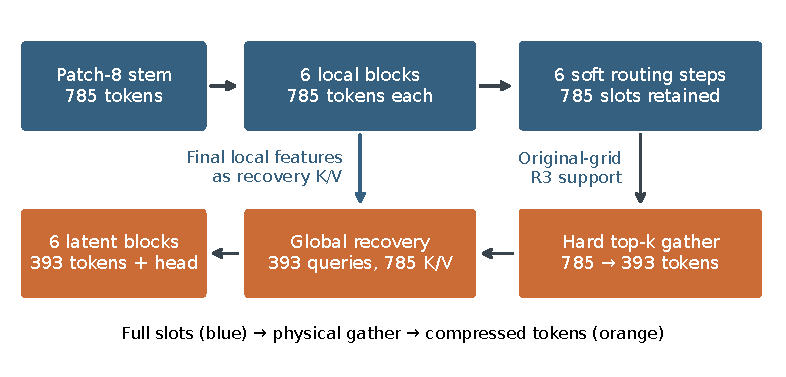
\includegraphics[width=\linewidth]{figures/architecture.pdf}
\caption{\mn{} at 224 pixels. Soft spatial transport keeps the full grid; the
exact-budget gather is the first physically shorter tensor. Recovery reads
the final full-grid local features, after which global reasoning uses 392
patch carriers. Counts exclude CLS.}
\label{fig:architecture}
\end{figure}

\subsection{Spatial mass routing}
Index patch $i$ by its original-grid coordinate $u_i$. At routing step
$\ell$, donor and receiver sets $A_\ell,B_\ell$ are disjoint, and donor $i$
may route only to
\begin{equation}
 \mathcal E_i^{(\ell)}(R)=\{j\in B_\ell:\|u_i-u_j\|_2\le R\}.
 \label{eq:support}
\end{equation}
The main model uses $R=3$. Coordinates stay tied to original slots throughout
routing. The global control removes this constraint; the flattened control
uses a width-8 window in row-major sequence order.

A learned $384\!\to\!64$ projection produces normalized metrics $z_i$. On
eligible edges,
\begin{equation}
 s_{ij}=\langle z_i,z_j\rangle/\tau,\quad
 q_{ij}=\frac{\exp s_{ij}}{\sum_{r\in\mathcal E_i}\exp s_{ir}},\quad
 a_{ij}=g_iq_{ij},
 \label{eq:routing}
\end{equation}
where $g_i$ is a soft donor decision. Following
\citet{sujianlin2024topk}, a monotone relaxation applies a data-dependent
threshold $\theta$ after sorting,
\begin{equation}
 g_i=F(\alpha\bar e_i-\theta),\qquad \sum_i g_i\approx k_\ell,
 \label{eq:softtopk}
\end{equation}
with row energy $e_i=\sum_j\exp s_{ij}$, $\alpha=30$, and the scheduled donor
budget $k_\ell$. This replaces serial top-$k$ decisions with a parallel soft
mask; it does not make the later gather indices differentiable.

Each slot carries mass $m_i$, initialized to one. A transport step preserves a
donor feature and transfers a fraction of its mass into receiver features:
\begin{align}
 m'_i&=m_i(1-\textstyle\sum_j a_{ij}), & X'_i&=X_i,\nonumber\\
 m'_j&=m_j+\textstyle\sum_i a_{ij}m_i, &
 X'_j&=\frac{m_jX_j+\sum_i a_{ij}m_iX_i}{m'_j}.
 \label{eq:transport}
\end{align}
The implementation clamps residual fractions and denominators. Sparse
neighbor lists restrict scored edges, but the released initialization still
constructs a dense adjacency buffer; our claim concerns learned routing
support, not linear memory for the whole implementation.

\subsection{Exact budget, recovery, and mass-aware attention}
For compression factor $\lambda$, the carrier count is
\begin{equation}
 K=N-\left\lfloor N(\lambda-1)/\lambda\right\rfloor.
 \label{eq:budget}
\end{equation}
The model hard-gathers the $K$ largest-mass patches. At $224^2$ and
$\lambda=2$, $N=784$ and $K=392$. A straight-through factor
$1+g-\operatorname{stopgrad}(g)$ on selected features sends gradients to the
continuous scores while hard indices execute the budget. Selected carriers
$Q$ then recover full-grid evidence through
\begin{equation}
 Y=Q+\operatorname{CrossAttn}(Q,H^{(6)},H^{(6)}),
 \label{eq:recovery}
\end{equation}
and six latent blocks process $K$ patches plus CLS.

Carrier mass enters latent attention as proportional attention:
\begin{equation}
 \operatorname{Attn}(Q,K,V;m)=
 \operatorname{softmax}\!\left(\frac{QK^\top}{\sqrt{d_h}}
 +\mathbf 1\log(m)^\top\right)V.
 \label{eq:mass-attn}
\end{equation}
The bias is rank one across queries. With
$\widehat Q=[Q,\sqrt{d_h}\mathbf1]$ and $\widehat K=[K,\log m]$, standard
scaled dot-product attention on $(\widehat Q,\widehat K,V)$ has exactly the
same logits. Padding the added head dimension to a multiple of eight lets the
released operator call unmodified FlashAttention. The reported ImageNet
checkpoints instead use PyTorch fused scaled-dot-product attention with an
additive mask; the FlashAttention path is validated separately by
forward/backward parity tests and is not credited with their runtime.

\section{Experimental Protocol}
\label{sec:setup}

\subsection{Data, optimization, and run identity}

We analyze an ImageNet-1k classification campaign with seed 42. Evaluation
uses the 50,000-image validation split and reports top-1 accuracy of the
exponential moving average (EMA) model. Every available training summary row
was matched to its final per-epoch EMA validation line in the launcher log:
2,419 rows across 17 runs with recorded epochs. There are 18 launched runs in
total: 16 complete schedules, one partial curriculum snapshot, and one
512-pixel \mn{} run with no completed epoch in the supplied record.
Checkpoint-verification receipts are present, but the weights themselves
were not transferred with the campaign packet. This audit verifies the
recorded outcomes; it is not an independent checkpoint re-evaluation.

The 224-pixel runs train from scratch for 150 or 300 epochs, using AdamW,
cosine learning-rate decay, five warmup epochs (twenty for the warmup probe),
weight decay 0.05, gradient
clipping at 1.0, label smoothing 0.1, Mixup 0.8, CutMix 1.0, RandAugment, and
random erasing probability 0.25. The base learning rate is $5\times10^{-4}$;
a separate \mn{} arm uses $7.5\times10^{-4}$. The higher-rate arm supplies
the 300-epoch \mn{} checkpoint. Therefore the final dense-versus-\mn{}
comparison is a comparison of selected configurations, while the geometry
comparison uses matched learning rates. No teacher distillation is enabled.
Appendix~\ref{app:recipe} gives the recipe and auxiliary-logit schedule.

The effective global batch is 1,024 throughout the recorded campaign. The
384/512-pixel fine-tunes use four-step gradient accumulation:
$32\times8\times4=1024$ for the dense 384-pixel run and
$64\times4\times4=1024$ for the other fine-tunes. Each fine-tune epoch contains
5,004 per-rank microsteps and 1,251 optimizer steps. Counting microsteps as
optimizer steps would incorrectly suggest a fourfold batch reduction.
Different world sizes and microbatches still produce different execution
and sample-grouping conditions; effective batch equality alone does not
establish bitwise equivalence.

\subsection{Resolution adaptation and checkpoint selection}

Three 384-pixel runs fine-tune the corresponding 300-epoch EMA weights for
30 epochs, using learning rate $10^{-5}$, minimum rate $10^{-6}$, one warmup
epoch, weight decay $10^{-8}$, and no Mixup or CutMix. EMA decay changes from
0.99996 to 0.9996. The \mn{} arms either retain $R=3$ or use
$R=3\times384/224\approx5.143$. The latter tests a particular proportional
radius scaling; it is not a complete radius search. Bicubic validation
preprocessing uses crop percentage 0.9 at 224 pixels and 1.0 for the
fine-tunes. The completed 512-pixel dense result follows its 384-pixel
checkpoint; there is no completed paired \mn{} result at that resolution.

We report both the best observed EMA top-1 and the final-epoch EMA top-1.
Best checkpoints are selected on the same validation split used for
reporting, so these scores are not independent held-out estimates of model
selection. Epoch indices start at zero. All completed-run comparisons use
actual summary headers rather than fixed column positions, because the
summary schema changes with enabled diagnostics. Runs with a teardown error
after a complete recorded schedule are distinguished from unfinished runs.

\subsection{Post-training compression and timing}

The accuracy sweep applies ToMe and PiToMe to the dense EMA checkpoint
without additional training, and changes \mn{}'s carrier budget without
retraining each point. Thus \mn{} has been trained with its native
compression, whereas the dense backbone was trained without merging. This
is a deployment comparison of available checkpoints, not an isolation of the
routing rule under identical training. We distinguish a 224-pixel checkpoint
evaluated at a new resolution from a checkpoint fine-tuned at that resolution.
Repeated successful sweep records are resolved by latest timestamp, not
highest accuracy. All included accuracy cells use the full validation split. Training-summary
validation uses 64 images per rank. For sweeps from the 224-pixel checkpoints,
\mn{} and ToMe use batch 128 and PiToMe uses batch 256; the final 384-pixel
fine-tuned curves use batch 256 for all three. The separate fine-tuned gate
uses batch 384. These batch distinctions matter for the soft-routing
implementation and are retained in the evidence ledger.

The 224-pixel efficiency experiment uses one H20-3e, synthetic inputs, batch
64, fp16 autocast, 30 warmup iterations and 50 measured iterations. It records
CUDA-event medians and interquartile ranges (IQRs); training cells include
forward, loss, backward and AdamW update. Device isolation is checked around
the measurements. The separate radius-3 benchmarks at 384 pixels use the
same thirty-warmup/fifty-measurement protocol at batches 64 and 128.
These are model-execution timings, excluding image loading,
and do not estimate end-to-end training time on eight GPUs. Training-log
throughput is excluded because the training machine was shared.

A later 384-pixel benchmark uses batch 64, ten warmup and 30 measured
iterations, random model initialization and synthetic inputs. It records
achieved token counts, but disables ToMe proportional attention, whereas the
accuracy sweep uses it. We retain these latency measurements as a separate
configuration-specific experiment and do not attach accuracy coordinates to
them. Final token counts also require care: the accuracy sweep counts patches,
while this timing harness counts the class token as well.

\section{Results}
\label{sec:results}

\subsection{Primary matched-budget comparison}
Table~\ref{tab:main} fixes the final budget at 392 patches, excluding CLS. The
\mn{} row is the 50,000-image re-evaluation (81.360\%); its training summary
reports a best EMA value of 81.368\%. Dense DeiT-S/8 reaches 82.246\%, and
post-training ToMe reaches 81.932\%. Thus the current evidence establishes a
learnable physical bottleneck, but not a stronger accuracy frontier. The
matched DTEM score and common-protocol systems cells remain explicit blanks.

\begin{table}[t]
\caption{ImageNet-1K at 224 pixels and a 392-patch target. Accuracy is percent.
Blank cells are requested measurements, not zero values or estimates.}
\label{tab:main}
\centering\footnotesize
\setlength{\tabcolsep}{3.2pt}
\begin{tabular}{llrr}
\toprule
Method & Checkpoint / path & Final patches & Top-1 (\%) \\
\midrule
DeiT-S/8 & trained dense & 784 & 82.246 \\
DeiT-S/8 + ToMe & post-training & 392 & 81.932 \\
DeiT-S/8 + PiToMe & post-training & 392 & 81.742 \\
\mn{} ($R=3$) & trained bottleneck & 392 & 81.360 \\
DTEM-p8 & common-recipe adaptation & 392 & \pendingvalue \\
\bottomrule
\end{tabular}

\end{table}

\subsection{Does the spatial prior help?}
\label{sec:cifar-seeds}
The 150-epoch ImageNet controls isolate routing support at learning rate
$5\times10^{-4}$. Radius 3 reaches 78.888\%, improving over global routing by
1.670 points and flattened windows by 0.598 (Table~\ref{tab:geometry}). Radius
2 is only 0.054 points higher, so one seed does not identify an optimal radius.
The global arm is an architectural control with \mn{}'s local/latent split,
not a reproduction of DTEM.

\begin{table}[t]
\caption{ImageNet routing controls. All rows use the same 150-epoch recipe;
accuracies are single-seed EMA top-1.}
\label{tab:geometry}
\centering\small
\begin{tabular}{lrrr}
\toprule
Routing / probe & LR ($10^{-4}$) & Best (\%) & Final (\%) \\
\midrule
Global & $5.0$ & 77.218 & 77.216 \\
Flat window 8 & $5.0$ & 78.290 & 78.278 \\
Spatial $R=2$ & $5.0$ & 78.942 & 78.942 \\
Spatial $R=3$ & $5.0$ & 78.888 & 78.888 \\
\bottomrule
\end{tabular}

\end{table}

Radius changes both geometry and candidate count. We therefore repeat the
comparison on CIFAR-100 with a receiver permutation that preserves each
realized receiver degree. Across three seeds, radius 3 ranks first under both
the historical batch-normalized threshold selector and a corrected per-sample
selector (Table~\ref{tab:cifar-seeds}). Every one of the 18 paired radius-3
minus control differences is positive. Against the degree-matched control,
the mean gains are $1.42\pm0.30$ and $1.19\pm0.13$ points, respectively. These
runs support a locality effect beyond degree, but do not transfer ImageNet
uncertainty.

\begin{table}[t]
\caption{CIFAR-100 epoch-199 EMA top-1 (\%), mean $\pm$ sample standard
deviation over seeds 42, 43, and 44.}
\label{tab:cifar-seeds}
\centering\footnotesize
\setlength{\tabcolsep}{3.4pt}
\begin{tabular}{lrrrr}
\toprule
Selector & Global & Flat 8 & Degree-matched & $R=3$ \\
\midrule
Historical selector & 68.48$\pm$0.10 & 69.29$\pm$0.54 & 69.17$\pm$0.62 & 70.59$\pm$0.88 \\
Rowwise selector & 68.77$\pm$0.32 & 69.64$\pm$0.80 & 69.21$\pm$0.75 & 70.41$\pm$0.67 \\
\bottomrule
\end{tabular}

\end{table}

Table~\ref{tab:ablation-map} ties each mechanism claim to a control. The two
remaining component interventions require only one inference pass of the
collaborator-held final checkpoint; they are diagnostic ablations rather than
separately trained architectures.

\begin{table}[t]
\caption{Claim-to-ablation map. ``Done'' rows contain complete experiments.}
\label{tab:ablation-map}
\centering\footnotesize
\setlength{\tabcolsep}{3pt}
\begin{tabular}{p{0.24\linewidth}p{0.39\linewidth}p{0.25\linewidth}}
\toprule
Claim & Control & Result \\
\midrule
2-D routing & global, flat, $R=2/3$ & Done; Table~\ref{tab:geometry} \\
Locality beyond degree & receiver permutation & $+1.42\pm0.30$ points \\
Selector dependence & historical vs per-sample & $R=3$ first under both \\
Budget behavior & 20 matched token settings & ToMe higher in 20/20 \\
Mass-aware attention & set $\log m$ bias to zero & \pendingresult{score} \\
Full-grid recovery & bypass cross-attention & \pendingresult{score} \\
\bottomrule
\end{tabular}
\end{table}

\subsection{Long schedules, resolution, and budgets}
At 300 epochs, \mn{} trails dense DeiT-S/8 by 0.878 points at 224 pixels
(Table~\ref{tab:resolution}). Fine-tuning narrows this gap to 0.394 at 384
pixels; at 512 pixels the gap is 0.450, so the three points do not support a
monotonic convergence claim. Different \mn{} radii are used across this
ladder and the 512-pixel arm descends from the radius-scaled 384 checkpoint.

\begin{table}[t]
\caption{Best EMA top-1 across resolution schedules. The gap is \mn{} minus
dense in percentage points.}
\label{tab:resolution}
\centering\small
\begin{tabular}{llrrr}
\toprule
Pixels & Schedule & DeiT-S/8 (\%) & MergeNet (\%) & Gap (pp) \\
\midrule
224 & 300 scratch & 82.246 & 81.368 & -0.878 \\
384 & 300+30 & 82.976 & 82.582 & -0.394 \\
512 & 300+30+15 & 83.068 & 82.618 & -0.450 \\
\bottomrule
\end{tabular}

\end{table}

Changing only the evaluation-time carrier budget gives \mn{} top-1 values of
81.380, 81.360, 81.074, 80.850, and 80.228\% at 523, 392, 314, 262, and 196
patches. ToMe applied to the dense checkpoint is higher at every one of these
224-pixel budgets, with gaps from 0.572 to 1.524 points; the same ordering
holds at all five 384-pixel budgets. This is a clear negative result for the
current end-to-end model. It is not a controlled comparison of training
objectives, because ToMe starts from the stronger dense checkpoint. Detailed
curves, optimizer probes, and complete schedules are in the appendix.

\subsection{Efficiency}
\label{sec:systems}

At 224 pixels, \mn{} passes 392 rather than 784 patches to the latent
stage and requires an estimated 14.13 GMAC per image, compared with
22.41 GMAC for dense DeiT-S/8, a 37.0\% reduction. The estimate excludes
indexing and data movement; Table~\ref{tab:a100-efficiency} measures their
combined effect with the rest of the implementation on an A100.

Compilation lowers the measured \mn{} batch-64 latency from
36.30 to 27.24\,ms, a 25.0\% reduction on the tested A100 configuration.
Compiled ToMe takes 27.22\,ms; peak allocated memory is 0.627\,GiB
for \mn{} and 0.614\,GiB for ToMe. Table~\ref{tab:a100-efficiency}
and Figure~\ref{fig:a100-efficiency} report both execution modes.
These model-only benchmarks use random weights and synthetic inputs;
Appendix~\ref{app:followup} specifies the measurement and compilation settings.

\begin{table}[H]
\caption{Synthetic A100 inference at 224 pixels with fp16 autocast
and random weights. B1/B64 denote batch sizes 1 and 64; memory is
batch-64 peak allocated and reserved GiB. The eager \mn{} B1 range
spans two independent run medians.}
\label{tab:a100-efficiency}
\centering\footnotesize
\setlength{\tabcolsep}{3.5pt}
\begin{tabular}{lrr}
\toprule
Model & 224 px (ms) & 384 px (ms) \\
\midrule
Dense DeiT-S/8 & 30.09 & 109.43 \\
ToMe, proportional attention on & 34.42 & 133.36 \\
ToMe, proportional attention off & 29.71 & 96.05 \\
MergeNet $R=3$ & 49.16 & 144.97 \\
MergeNet $R=3$, BNHD & 46.56 & 138.11 \\
MergeNet $R=5.143$ & -- & 218.25 \\
MergeNet $R=5.143$, BNHD & -- & 211.40 \\
\bottomrule
\end{tabular}

\end{table}

\begin{figure}[H]
\centering
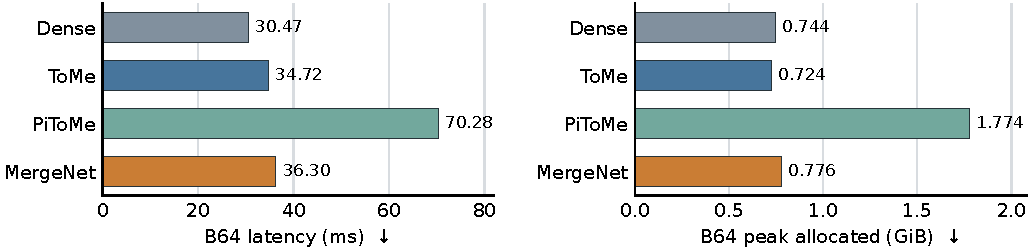
\includegraphics[width=\linewidth]{figures/a100_efficiency.pdf}
\caption{Batch-64 A100 inference with random weights.
Solid bars denote eager execution; hatched bars denote compiled execution.
Latency and peak allocated memory use the measurements in
Table~\ref{tab:a100-efficiency}; lower is better.}
\label{fig:a100-efficiency}
\end{figure}

A separate high-resolution benchmark on an H20 measures 136.54\,ms
for \mn{} and 170.61\,ms for dense DeiT-S/8 at 384 pixels and batch 64.
Peak allocated memory is 2.969 and 1.983\,GiB, respectively.
This operating point illustrates a latency reduction alongside a larger
memory footprint. Appendix~\ref{app:highres-efficiency} reports the
training and inference measurements under that hardware setup.

\section{Discussion and Limitations}

The results distinguish an internal architectural improvement from a
competitive compression system. Original-grid support improves this
architecture relative to its own unconstrained router. Yet the full model
loses accuracy to the selected dense baseline, its 224-pixel implementation
is slower in guarded synthetic tests, and post-training ToMe provides a
stronger accuracy baseline at every matched budget in the sweep. These
findings motivate revisiting the computation path and evaluation protocol;
they do not show that learning a merge criterion is intrinsically inferior.

The evidence is limited in several ways. All training runs use seed 42, and
the validation set serves both checkpoint selection and reporting. We have
no across-seed uncertainty estimate or per-image predictions for paired
significance tests. Geometry and candidate cardinality remain coupled. The
300-epoch \mn{} configuration benefits from an explicit learning-rate screen,
while the dense baseline is not subjected to an equally broad screen. The
$\lambda=4$ training variant changes multiple architectural parameters, and
test-time budget changes do not replace a clean training-budget ablation.
The curriculum and paired 512-pixel result are incomplete at capture time.

The experiment artifacts also bound reproducibility. Raw metrics, resolved
arguments, launch records, environment information, benchmark scripts and
checkpoint receipts are available in the campaign packet. Actual trained
weights were not transferred for this audit, and a release commit alone does
not capture every change in the collaborator's working tree. The companion
analysis preserves the source identities and distinguishes recorded results
from independent operator diagnostics. The training environment uses PyTorch
2.7.1 with CUDA 11.8, timm 0.9.11 and FlashAttention 2.7.3, which differs from
the local release's pinned environment. CPU profiles and H20 synthetic timings
cannot establish performance on every accelerator or under deployment load.
The ToMe attention-policy mismatch must be resolved before a joint frontier
is reported.

The most informative next experiments follow directly from these limits.
First, reevaluate transferred EMA weights with explicit batch composition and
a common accuracy/timing configuration, recording exact per-layer shapes.
Second, test a numerically stable, per-sample soft-selection operator and
separate its effect from a change in training or evaluation batch. Third,
repeat the global, flattened and radius-3 controls at additional seeds and
include a degree-matched spatial control. System optimizations should then
be evaluated with forward/backward parity and complete-model timing. These
experiments would test concrete explanations for the observed gaps; merely
extending a schedule based on a short terminal slope would not.

\section{Conclusion}

\mn{} combines continuous spatial mass transport with an exact-budget gather,
so a learned routing policy feeds a physically shorter latent sequence in the
same forward path. The original-grid prior consistently improves routing
controls, including a degree-matched three-seed study, and accumulated carrier
mass admits an exact FlashAttention-compatible key-bias construction. Current
ImageNet results also expose the remaining gap: the model does not yet exceed
dense DeiT-S/8 or post-training ToMe in accuracy, and its deployment frontier
awaits common-protocol checkpoint measurements. This evidence supports the
compression boundary and spatial-routing mechanism while defining a precise,
testable path to a stronger system result.

\FloatBarrier
\bibliographystyle{plainnat}
\bibliography{references}
\clearpage
\appendix
\section{Training Recipe and Evidence Inventory}
\label{app:recipe}

Table~\ref{tab:recipe} summarizes the resolved run arguments. The base width
is 384 with six heads and MLP expansion four. Stochastic depth is configured
at 0.1; \mn{} constructs separate local and latent ramps, unlike a single
twelve-block dense ramp. The global and flattened routing controls use their
dense/historical scoring paths, while radius-2/3 routing uses the sparse
spatial backend; the routing support and its numerical implementation should
therefore both be recorded. EMA validation replaces raw-model metrics before
the summary row is written, so \texttt{eval\_top1} is an EMA metric.

\begin{table}[h]
\centering\small
\begin{tabular}{lll}
\toprule
Setting & 224-pixel scratch & 384/512-pixel fine-tune\\
\midrule
Epochs & 150 or 300 & 30 at 384; 15 at 512\\
Effective global batch & 1024 & 1024\\
Optimizer & AdamW & AdamW\\
Learning rate & $5\!\times\!10^{-4}$ or $7.5\!\times\!10^{-4}$ & $10^{-5}$\\
Minimum learning rate & $10^{-5}$ & $10^{-6}$\\
Weight decay & 0.05 & $10^{-8}$\\
Warmup epochs & 5 (probe: 20) & 1\\
Warmup learning rate & $10^{-6}$ & $10^{-6}$\\
EMA decay & 0.99996 & 0.9996\\
Mixup / CutMix & 0.8 / 1.0 & 0 / 0\\
Label smoothing & 0.1 & 0.1\\
Random erasing & 0.25 & 0.25\\
RandAugment & \texttt{rand-m9-mstd0.5-inc1} & same\\
Gradient clip norm & 1.0 & 1.0\\
Validation crop percentage & 0.9 & 1.0\\
\mn{} auxiliary-logit weight & ramp to 0.05 & 0.05\\
Teacher / feature / routing distillation & disabled & disabled\\
\bottomrule
\end{tabular}
\caption{Main recipe. Launch records take precedence over configuration-file
defaults, especially for microbatch size and gradient accumulation.}
\label{tab:recipe}
\end{table}

\paragraph{Classifier implementation.}
The main configuration uses patch size 8, width 384, six heads, six local
blocks, and six latent blocks. At 224 pixels this gives 784 patch slots; the
local attention band extends 16 sequence positions on either side of a patch
query, while the CLS query attends globally. Spatial routing uses radius 3,
a $384\to64$ metric projection, similarity temperature 1, and input-gradient
scale 0.1 for the metric. At compression factor 2, the six soft donor budgets
are $(65,65,65,65,65,67)$ and the hard gather retains 392 patches. There is
no further merging in the latent encoder. Training partitions donors and
receivers randomly for each image; evaluation alternates deterministic
odd/even partitions across routing steps.

\paragraph{Selection and tracing.}
The threshold-based soft top-$k$ uses scale 30 and normalizes row energies by
their maximum-minus-minimum range across the current minibatch. Thus soft
selection can depend on batch companions; the released operator has no guard
for a zero range. The final hard-gather indices are detached and selected
carriers are sorted by a detached, mass-weighted center of their flattened
source indices. The default center-tracing mode does not retain a full source
membership matrix. Spatial scoring uses sparse neighbor lists, although
model initialization constructs a dense Boolean adjacency buffer.

During training, an auxiliary readout averages full-grid features using
soft-selection weights, applies the shared classification head, and adds its
weighted logits to the latent CLS logits. It is absent at evaluation and is
not a separate auxiliary loss. The 150-epoch \mn{} runs start this
contribution at epoch 10
and ramp it over 10 epochs; the 300-epoch run uses epoch 20 and a 20-epoch
ramp. Fine-tunes enable weight 0.05 from the start. The
recorded environment is Python 3.10.20, PyTorch 2.7.1+cu118, torchvision
0.22.1+cu118, timm 0.9.11, FlashAttention 2.7.3 and Triton 3.3.1 on H20-3e
GPUs. Both four and eight ranks divide 50,000, avoiding validation-sampler
padding for this split. Other world sizes require a separate check.

Three nominal launcher failures occurred after complete metric histories:
the 150-epoch DeiT-S/16, the compound $\lambda=4$ run, and dense 512-pixel
fine-tuning. Complete summaries and supplied checkpoint receipts distinguish
them from early failures. Receipts record checks on another machine, not
weights independently loaded in this audit. The $\lambda$ curriculum and
512-pixel \mn{} fine-tune are now complete 150-epoch and 15-epoch records.
The weight-decay probe was abandoned at 140/150. The DeiT-initialized and
progressive-latent runs are complete 150-epoch records.

\begin{table}[h]
\centering\footnotesize
\begin{tabular}{lrlr}
\toprule
Run ID & Epochs & Status & Best top-1 \\
\midrule
\texttt{s2\_deit\_p16\_150e} & 150/150 & Complete & 77.196 \\
\texttt{s2\_deit\_p8\_150e} & 150/150 & Complete & 79.992 \\
\texttt{s2\_mn\_flat\_w8\_150e} & 150/150 & Complete & 78.290 \\
\texttt{s2\_mn\_global\_150e} & 150/150 & Complete & 77.218 \\
\texttt{s2\_mn\_l4\_150e} & 150/150 & Complete & 78.366 \\
\texttt{s2\_mn\_r2\_150e} & 150/150 & Complete & 78.942 \\
\texttt{s2\_mn\_r3\_150e} & 150/150 & Complete & 78.888 \\
\texttt{s2\_mn\_r3\_lr75\_150e} & 150/150 & Complete & 79.316 \\
\texttt{s3\_deit\_p16\_300e} & 300/300 & Complete & 79.692 \\
\texttt{s3\_deit\_p8\_300e} & 300/300 & Complete & 82.246 \\
\texttt{s3\_mn\_r3\_lr75\_300e} & 300/300 & Complete & 81.368 \\
\texttt{s3\_deit\_p8\_ft384\_30e} & 30/30 & Complete & 82.976 \\
\texttt{s3\_mn\_r3\_ft384\_30e} & 30/30 & Complete & 82.582 \\
\texttt{s3\_mn\_r5\_ft384\_30e} & 30/30 & Complete & 82.574 \\
\texttt{s4\_mn\_lamcurr\_150e} & 150/150 & Complete & 79.310 \\
\texttt{s4\_mn\_warm20\_150e} & 150/150 & Complete & 79.238 \\
\texttt{s4\_deit\_ft512\_15e} & 15/15 & Complete & 83.068 \\
\texttt{s4\_mn\_ft512\_15e} & 15/15 & Complete & 82.618 \\
\texttt{s5\_mn\_dp07\_150e} & 150/150 & Complete & 79.534 \\
\texttt{s5\_mn\_lr1e3\_150e} & 150/150 & Complete & 79.350 \\
\texttt{s5\_mn\_wd03\_150e} & 140/150 & Partial & 79.054 \\
\texttt{s6\_deitB\_p16\_300e} & 300/300 & Complete & 80.442 \\
\texttt{s7\_mn\_deitinit\_150e} & 150/150 & Complete & 80.574 \\
\texttt{s7\_mn\_proglatent\_150e} & 150/150 & Complete & 79.392 \\
\bottomrule
\end{tabular}

\caption{Status through the September 23 packet. The abandoned weight-decay
metric is included for accounting only and is not an endpoint. The DeiT-B best score is a
pre-overfitting peak (Appendix~\ref{app:deitb}). The companion data retain
full precision and source summary lines.}
\label{tab:runs}
\end{table}
\FloatBarrier

\subsection{Initialization and Latent-Compression Diagnostics}

Table~\ref{tab:stage7-diagnostics} uses the completed drop-path-0.07 run as
the 150-epoch scratch control. Initializing \mn{} from the 300-epoch
DeiT-S/8 checkpoint raises best EMA top-1 by 1.040 points. This result shows
initialization sensitivity, not equal-total-compute superiority: the source
representation already consumed 300 training epochs, the experiment has one
seed, and its 80.574\% endpoint remains below both the 300-epoch scratch
\mn{} result (81.368\%) and its dense source (82.246\%). The original
first-launch loading log was not delivered after a host migration; the
record retains a contemporaneous 152-loaded/25-missing receipt and the early
learning curve, so we treat this as a diagnostic rather than a primary causal
result.

The progressive-latent variant adds 192 latent-stage merges and reaches
79.392\%, 0.142 points below the same control. It changes the final configured
budget from approximately 392 to 200 patches, so it is an
accuracy--compression probe rather than a matched-budget test of gradual
versus abrupt scheduling. With one seed, the result establishes no observed
gain but does not establish a statistically resolved degradation. Training-log
throughput is not used as deployment latency.

\begin{table}[h]
\caption{Completed 150-epoch Stage-7 diagnostics, all with seed 42 and
drop-path 0.07. Deltas use the scratch control in the first row.}
\label{tab:stage7-diagnostics}
\centering\small
\begin{tabular}{llrr}
\toprule
Variant & Setting / change from control & Best (\%) & $\Delta$ (pp) \\
\midrule
Scratch control & drop-path 0.07 & 79.534 & 0.000 \\
DeiT initialization & initialize from DeiT-S/8 300e & 80.574 & +1.040 \\
Progressive latent & 192 additional latent merges & 79.392 & -0.142 \\
\bottomrule
\end{tabular}

\end{table}

\section{Detailed Budget and Timing Comparisons}
\label{app:latency}

Table~\ref{tab:sweepdetail} gives the values behind the main accuracy panels.
The \mn{} checkpoint uses radius 3 at 224 pixels and radius 5.143 after
384-pixel fine-tuning. Final patch budgets match within a row, but layerwise
attention and MLP inputs do not. ToMe and PiToMe shorten sequences within
successive blocks, while \mn{} gathers once between stages. The companion
CSV also contains the two resolution-transfer panels using 224-pixel
checkpoints without fine-tuning.

\begin{table}[h]
\centering\small
\begin{tabular}{lrrrrr}
\toprule
Checkpoint / pixels & Patches & MergeNet & ToMe & PiToMe & $\Delta$ ToMe \\
\midrule
224 trained / 224 & 523 & 81.380 & 82.038 & 81.876 & +0.658 \\
224 trained / 224 & 392 & 81.360 & 81.932 & 81.742 & +0.572 \\
224 trained / 224 & 314 & 81.074 & 81.814 & 81.560 & +0.740 \\
224 trained / 224 & 262 & 80.850 & 81.830 & 81.500 & +0.980 \\
224 trained / 224 & 196 & 80.228 & 81.752 & 81.206 & +1.524 \\
384 tuned / 384 & 1537 & 82.500 & 82.868 & 82.658 & +0.368 \\
384 tuned / 384 & 1152 & 82.562 & 82.866 & 82.534 & +0.304 \\
384 tuned / 384 & 923 & 82.230 & 82.800 & 82.452 & +0.570 \\
384 tuned / 384 & 770 & 82.002 & 82.792 & 82.334 & +0.790 \\
384 tuned / 384 & 576 & 81.300 & 82.742 & 82.296 & +1.442 \\
\bottomrule
\end{tabular}

\caption{Top-1 percentages at equal final patch counts; $\Delta$ is ToMe minus
\mn{} in percentage points. These values cannot be paired with
Table~\ref{tab:latency384} to construct an accuracy--latency frontier.}
\label{tab:sweepdetail}
\end{table}

\begin{table}[h]
\centering\small
\begin{tabular}{rrrrrr}
\toprule
ToMe patches & MN patches & ToMe ms & MN ms & ToMe GiB & MN GiB \\
\midrule
1536 & 1538 & 147.30 & 178.17 & 2.793 & 3.619 \\
1151 & 1152 & 129.81 & 155.25 & 2.764 & 3.564 \\
922 & 923 & 122.44 & 143.02 & 2.746 & 3.721 \\
769 & 770 & 118.17 & 136.59 & 2.738 & 3.719 \\
575 & 576 & 106.45 & 129.38 & 2.723 & 3.557 \\
\bottomrule
\end{tabular}

\caption{Separate 384-pixel synthetic latency experiment: batch 64, H20-3e,
fp16 autocast, random initialization, \mn{} radius 5.143, and ToMe
proportional attention disabled. Patch counts exclude the class token here.
Memory is peak \emph{reserved} GiB, unlike the historical 224-pixel record,
which reports peak allocated memory.
Token-counting hooks remain active during timing.}
\label{tab:latency384}
\end{table}

At the approximately half-size operating point, ToMe processes 1,151 patches
and \mn{} 1,152, taking 129.810 and 155.255\,ms respectively. These times do not
prove a joint ordering for the accuracy sweep's ToMe setting. A common
harness should use exactly 1,152 patches with proportional attention enabled,
verify the checkpoint and preprocessing, and remove shape hooks before
timing. An earlier latency benchmark silently clamped several requested
ToMe budgets to the same achieved count; those obsolete cells are excluded.

Separate 384-pixel radius-3 benchmarks remain distinct from the radius-5.143
sweep. Speed percentages at different batch sizes, radii or harness settings
should not be averaged into an unexplained range. Peak reserved memory and
peak allocated memory also measure different quantities.

\section{Evidence and Reproduction Boundaries}

The artifact subset includes unmodified per-run summaries, resolved arguments
with host paths removed, launch-protocol extracts, sanitized successful sweep
records, audited benchmark tables, and source hashes. The CPU rebuild script
recomputes best/final metrics, resolves sweep records by timestamp, checks
numeric joins, and regenerates tables and figures. It never launches
training. Source and claim ledgers retain their literature retrieval dates;
the collaborator-packet audit was refreshed on September 21.
Company policy prevents ImageNet weight
transfer; independent ImageNet checkpoint re-evaluation is unavailable. The
September 23 packet additionally completes the two Stage-7 diagnostics.
The refreshed audit matches 3,354 of 3,560 summary rows to delivered EMA logs,
leaving 206 rows without corresponding log records
(Section~\ref{sec:setup}). Those rows are not discarded, but retain their
summary-only evidence status.

\section{DeiT-B/16 is not a usable scale anchor}
\label{app:deitb}

A 300-epoch DeiT-B/16 run at 224 pixels completes under the same global-batch
and seed protocol as the small-scale campaign, with drop-path 0.1 inherited
from the DeiT-S configurations. Table~\ref{tab:deitb} reports the peak and
final EMA scores. Train loss continues to fall while evaluation loss rises
after the peak at epoch 179. The final top-1, 78.566\%, is below our
DeiT-S/16 result of 79.692\% at the same 196-token budget. Published DeiT-B
300-epoch training uses drop-path 0.2. We therefore do not append this run
to the DeiT-S/8 table, and we do not launch a paired MergeNet-B comparison
from these weights.

\begin{table}[h]
\centering\small
\begin{tabular}{lrrr}
\toprule
Epoch & Train loss & Eval loss & EMA top-1 (\%) \\
\midrule
150 & 2.968 & 0.889 & 80.060 \\
179 (peak) & 2.808 & 0.895 & 80.442 \\
299 (final) & 2.348 & 1.095 & 78.566 \\
\bottomrule
\end{tabular}

\caption{DeiT-B/16, 300 epochs, drop-path 0.1. Peak and final scores must be
reported together; the peak is not a converged result.}
\label{tab:deitb}
\end{table}

\section{A Bounded Layout Optimization Experiment}
\label{app:layout}

We additionally test a single LocalAttention module on an A100-SXM4-80GB.
The original module constructs query/key/value tensors in
batch--head--token--channel order, then transposes and copies them for the
FlashAttention wrapper. An isolated variant constructs
batch--token--head--channel tensors directly and adjusts the global class-query
attention views and final reshape accordingly. It does not alter the
released model, load a checkpoint, or apply an optimizer update.

The test uses PyTorch 2.6.0+cu124 and FlashAttention 2.7.4.post1, width 384,
six heads, window radius 16, zero attention dropout, float32 parameters and
inputs, and fp16 autocast. Four batch-2 parity cases cover sequence lengths
785 and 2,305, global class attention on/off, and query/key normalization.
Outputs and input gradients are bitwise equal in these cases. Parameter
gradients are also equal except for the normalization case, whose maximum
relative $L_2$ error is $5.77\times10^{-7}$. This coverage does not establish
all-shape or dropout/RNG-preserving equivalence for a complete model.

\begin{table}[h]
\centering\small
\begin{tabular}{rrlrrr}
\toprule
Batch & Tokens & Mode & Original ms & Layout ms & Reduction range\\
\midrule
64 & 785 & Forward & 1.5600 & 1.0448 & 13.50--34.03\%\\
64 & 785 & Forward + backward & 5.1590 & 4.3999 & 14.68--25.64\%\\
16 & 2305 & Forward & 1.0318 & 0.9369 & 6.88--36.68\%\\
16 & 2305 & Forward + backward & 5.3740 & 4.9176 & 5.45--11.83\%\\
\bottomrule
\end{tabular}
\caption{Single-module A100 measurements. Times are medians of three round
medians, each with five warmups and twenty CUDA-event samples. The final
column is the range of paired-round time reductions, not a confidence
interval. Tokens include the class token. Backward includes a squared-output
loss and gradient clearing, with no optimizer.}
\label{tab:layout}
\end{table}

Measurement order alternates by round, and the harness requires an initially
empty device, establishes its CUDA process identity, then rejects a changed
process set at subsequent checks. All iteration samples and snapshots are
retained. The observed reductions support this local engineering direction,
but the round variation is appreciable. Both module instances are resident,
so their recorded memory peaks are not independent per-model memory
measurements. These results do not predict the full model's speedup, validate
an HBM-traffic estimate, transfer H20 timings to A100, or resolve the separate
ToMe attention-policy mismatch.

\clearpage
% Standalone appendix fragment. No additional packages or bibliography keys.
% All numbers are independently recomputed by cifar_audit/recompute.py.
\section{CIFAR-100 Pilot Study}
\label{app:cifar-spatial}

We retain a historical CIFAR-100 experiment as a limited diagnostic of the routing geometry.
The August campaign contains 60 new runs: two MergeNet configurations, five input sizes, and six routing settings (Global and Euclidean radii $R\in\{1,2,3,4,8\}$), all using seed 42.
The configurations have local/latent depths of $6/6$ with final compression ratio $\lambda=2$, or $4/8$ with $\lambda=4$; both use width 384, six heads, and $8\times8$ patches.
Each model was trained from scratch for 200 epochs without distillation.
Training used AdamW, learning rate $10^{-3}$, weight decay 0.05, a cosine schedule with 20 warmup epochs, effective batch size 200, and EMA decay 0.9998.
The primary endpoint is the final epoch-199 EMA top-1 accuracy on the 10,000-image CIFAR-100 test set.
The frozen local campaign protocol designated $R=3$ as the primary setting before the recorded training launches; this is an internal protocol record, not an external preregistration.
We keep that setting even though $R=2$ has a slightly higher mean.

The original images are $32\times32$ pixels and are resized to the listed input sizes.
Thus, this sweep changes the patch grid over upsampled images and does not test native high-resolution image content.
Evaluation used FP16 autocast and deterministic fast grouping, with batches of 200, 200, 200, 100, and 50 at sizes 160, 192, 224, 256, and 320, respectively.
Global and the finite-radius settings were trained in the same frozen implementation and share the non-routing configuration.
The additional Flat reference uses the historical flattened-window implementation with width parameter 8 and comes from ten earlier August runs.
Its recorded non-routing training arguments and dependency versions match, but its runtime code snapshot differs; three Flat runs resumed within their original jobs.
We therefore use Flat as a historical descriptive reference.

\begin{table}[htbp]
\centering
\small
\setlength{\tabcolsep}{4pt}
\begin{tabular}{lrrrrrr}
\hline
Configuration & Input & Global & Flat$^\dagger$ & $R=3$ & $\Delta$G & $\Delta$F \\
\hline
$6/6$, $\lambda=2$ & 160 & 67.80 & 68.79 & 69.42 & +1.62 & +0.63 \\
 & 192 & 69.42 & 69.93 & 70.85 & +1.43 & +0.92 \\
 & 224 & 69.50 & 70.53 & 70.53 & +1.03 & +0.00 \\
 & 256 & 69.50 & 70.12 & 71.03 & +1.53 & +0.91 \\
 & 320 & 69.85 & 70.81 & 71.42 & +1.57 & +0.61 \\
$4/8$, $\lambda=4$ & 160 & 65.29 & 66.69 & 67.92 & +2.63 & +1.23 \\
 & 192 & 69.87 & 69.75 & 71.27 & +1.40 & +1.52 \\
 & 224 & 68.21 & 69.87 & 70.52 & +2.31 & +0.65 \\
 & 256 & 67.35 & 68.30 & 69.40 & +2.05 & +1.10 \\
 & 320 & 66.05 & 67.08 & 68.83 & +2.78 & +1.75 \\
\hline
Mean & & 68.284 & 69.187 & 70.119 & +1.835 & +0.932 \\
\hline
\end{tabular}
\caption{Historical CIFAR-100 final-epoch EMA accuracy (\%) and $R=3$ deltas (percentage points) against Global ($\Delta$G) and Flat ($\Delta$F). Each row uses seed 42; the mean gives equal weight to the ten configuration--input pairs. $^\dagger$Flat is a historical reference with a different code snapshot. Input denotes the resized side length of native $32\times32$ images. These are observations under the stated evaluation batches and historical dense-score implementation.}
\label{tab:cifar-spatial-audit}
\end{table}

At the fixed $R=3$ setting, accuracy exceeds Global in all ten pairs, with a mean improvement of 1.835 percentage points.
Relative to historical Flat, nine pairs improve and one ties, with a mean difference of 0.932 points.
Across the complete sweep, the mean accuracies for Global and radii 1, 2, 3, 4, and 8 are 68.284, 68.774, 70.225, 70.119, 70.047, and 68.414\%, respectively.
Radii 2, 3, and 4 each exceed their matched Global control in all ten pairs.
These correlated, single-seed observations provide evidence that restricting routing neighborhoods can help in this particular setting; they do not establish statistical significance, native-resolution transfer, or superiority over external token-reduction methods.

The audit reconciled all 60 new endpoints and the ten Flat endpoints with raw 200-epoch summaries, completion receipts, and frozen manifests.
Archived full-test evaluations of the 60 new epoch-199 EMA checkpoints show identical generic- and fast-grouping logits; their accuracies differ from the training summaries in 31 cases by at most 0.02 points.
The table preserves the registered training-summary endpoint.
The initial historical audit checked receipt hashes and checkpoint presence, without freshly evaluating or rehashing all checkpoints.
The historical spatial implementation constructs a dense donor--receiver score matrix before masking, so these results do not validate the later sparse backend or its efficiency.
Section~\ref{sec:cifar-seeds} reports a later 12-run campaign with three seeds and a degree-matched control; those runs are independent trainings and are not substitutes for the table above.

\section{Independent Follow-up with Available Local Artifacts}
\label{app:followup}

Company policy prevents transfer of the ImageNet checkpoints. We therefore
separate two feasible follow-ups: architecture timing using random weights,
and prediction tests using existing, locally available CIFAR-100 weights.
Neither experiment independently reproduces the company ImageNet scores.

\subsection{A common A100 inference harness}

We compare dense DeiT-S/8, ToMe, and the canonical sparse-backend \mn{} on
an A100-SXM4-80GB using PyTorch 2.6.0+cu124, timm 0.9.11 and
FlashAttention 2.7.4.post1. All cells use batch 64, float32 parameters and
inputs, and fp16 autocast. The compressed models retain exactly 392 patches
at 224 pixels and 1152 at 384 pixels, excluding CLS. A diagnostic forward
records block outputs; all hooks are removed before timing. ToMe source
tracing is disabled. Proportional attention is explicitly controlled, with
its enabled setting matching the recorded accuracy protocol.

Each cell has ten warm-up iterations and thirty CUDA-event samples in each
of three rounds, reversing model order in the middle round. A selected-GPU
process guard requires an empty device before setup and only our process
during the experiment. Models are allocated and released sequentially.
Table~\ref{tab:followup-latency} reports the median of three round medians.
It measures model execution, excluding data loading, backward and updates.

\begin{table}[h]
\centering\small
\begin{tabular}{lrr}
\toprule
Model & 224 px (ms) & 384 px (ms) \\
\midrule
Dense DeiT-S/8 & 30.09 & 109.43 \\
ToMe, proportional attention on & 34.42 & 133.36 \\
ToMe, proportional attention off & 29.71 & 96.05 \\
MergeNet $R=3$ & 49.16 & 144.97 \\
MergeNet $R=3$, BNHD & 46.56 & 138.11 \\
MergeNet $R=5.143$ & -- & 218.25 \\
MergeNet $R=5.143$, BNHD & -- & 211.40 \\
\bottomrule
\end{tabular}

\caption{Independent synthetic A100 inference, batch 64. All weights are
randomly initialized; these are not trained-checkpoint frontier points.
BNHD changes the local-attention tensor layout. The 384-pixel radius-5.143
model has the same final patch budget as radius 3.}
\label{tab:followup-latency}
\end{table}

On this local hardware/software stack, the original \mn{} is slower than
dense DeiT at both resolutions. The BNHD change reduces complete-model
radius-3 time by about 5\%, considerably less than the isolated-module
improvement. The proportional-attention setting materially affects ToMe
latency. Thus neither the H20 crossover nor a ToMe timing measured with
proportional attention disabled should be treated as accelerator-independent
evidence. The A100 comparison changes the hardware and software stack
relative to the H20 experiment; it does not isolate a hardware-only cause.
No historical accuracy point is attached to these random-weight timings.

\subsection{Layout validation under a complete training graph}

The layout comparison uses identical weights and images, restored CPU and
CUDA random states, fresh per-sample routing, and zero dropout at both
224 and 384 pixels. With the dense routing reference backend, outputs,
input gradients and all parameter gradients are bitwise equal. With the
sparse backend and an unscaled squared-logit loss, the strict gradient
comparison fails; an unchanged-model repeat also fails, so these runs do
not isolate an error introduced by BNHD. Their input-gradient relative
errors are approximately 4.8\% and 16.3\%, respectively.

We retain these failed tests and add a fixed loss scale of 1024, unscaling
all gradients before comparison. The sparse-backend tests then pass the
predefined relative-$L_2$ limits of 0.002 for outputs and 0.003 for gradients.
Maximum parameter-gradient relative errors are below 0.0016; unchanged-model
repeat controls are below 0.0018. This diagnoses sensitivity of the unscaled
fp16 test and supports bounded layout parity. It does not establish long-run
training equivalence, eliminate sparse-kernel nondeterminism, or validate
arbitrary dropout and precision settings.

\clearpage
\section{Reserved Extensions and Outstanding Evidence}
\label{app:pending}
These are intentionally unfilled working-draft slots, not additional results.
Optional experiments may be omitted together with the associated claims.
Original observations and partial runs remain in the evidence inventory.

\subsection{Base-scale comparison}
\label{sec:pending-base}
\pendingslot{P09}{Establish a credible dense reference before a scale claim}{The
completed drop-path-0.1 DeiT-B run remains a reported negative observation.}

Specify matched Base-scale training and effective layerwise stochastic depth.
Diagnose the dense reference's overfitting before interpreting a MergeNet-B
comparison. A different regularization recipe is a new experiment, not a
correction that replaces the old result.
\begin{center}\small\begin{tabular}{lrrrr}\toprule
Arm & Seeds & Best EMA & Final EMA & Batch latency (ms)\\\midrule
New dense Base reference & \pendingvalue & \pendingvalue & \pendingvalue & \pendingvalue\\
Matched MergeNet-B & \pendingvalue & \pendingvalue & \pendingvalue & \pendingvalue\\
\bottomrule\end{tabular}\end{center}
\pendingtext

\subsection{Same-parent radius comparison at 512 pixels}
\label{sec:pending-radius}
\pendingslot{P10}{Separate radius from checkpoint ancestry}{Optional; the
existing 512-pixel result is valid for its recorded radius-5.143 parent.}

A radius-only inference comparison uses one checkpoint with other settings
fixed. A fine-tuning comparison initializes both radii from the same verified
384-pixel state and uses the same 15-epoch recipe. An EMA extraction from
the radius-3 checkpoint permits that branch, but comparing a new R3-parent
branch only to the old R5.143-parent branch still mixes parent and radius.
\begin{center}\small\begin{tabular}{lrrr}\toprule
512-pixel arm & Parent identity & Best EMA & Final EMA\\\midrule
Fixed radius & \pendingvalue & \pendingvalue & \pendingvalue\\
Scaled radius, same parent & \pendingvalue & \pendingvalue & \pendingvalue\\
\bottomrule\end{tabular}\end{center}
\pendingtext

\subsection{Weight-decay probe completion}
\label{sec:pending-wd}
\pendingslot{P11}{Complete only if a full weight-decay result is needed}{The
140/150 snapshot is neither a completed negative result nor a statistical null.}

If resumed, retain the original state and append epochs 140--149 without
duplicating earlier rows. Otherwise keep partial status and omit endpoint
claims. Not crossing a decision threshold is not statistical equivalence.
\begin{center}\small\begin{tabular}{lrrr}\toprule
Run & Completed epochs & Best EMA & Final EMA\\\midrule
Weight decay 0.03 & \pendingvalue & \pendingvalue & \pendingvalue\\
\bottomrule\end{tabular}\end{center}
\pendingtext

\subsection{Additional log and state receipts}
\label{sec:pending-receipts}
\pendingslot{P12}{Complete source-to-result linkage without transferring weights}{
Existing configurations and environment records need not be re-exported
unless actual execution differs.}

For each new result provide run ID, complete metrics, resolved arguments
including launcher overrides, startup/resume lines, actual code-file hashes
and environment versions. Evaluations and initialization also need checkpoint
digest, state key, epoch, EMA flag and tensor mapping or verification receipt.
Digests identify artifacts without sharing parameter values. If a receipt
cannot be disclosed, record that evidence boundary.

Some September 19 summaries extend past the copied logs. Missing segments
must be supplied or labeled summary-only. The companion audit identifies
exact gaps and excludes documented earlier attempts; CSV recalculation is
not checkpoint replay.
\begin{center}\small\begin{tabular}{lrrl}\toprule
Additional receipt & Expected epochs / key & Verified count & Digest\\\midrule
Curriculum missing EMA logs & 64--149 & \pendingvalue & \pendingvalue\\
MergeNet 512-pixel EMA logs & 0--14 & \pendingvalue & \pendingvalue\\
Initialization state / full mapping & raw / EMA & \pendingvalue & \pendingvalue\\
New run source manifest & per run & \pendingvalue & \pendingvalue\\
\bottomrule\end{tabular}\end{center}
\pendingtext

\end{document}
